\chapter{From BCS to conventional superconductors}\chaptertoc{}\label{chap:from bcs to conventional superconductors}

The last chapters were devoted to a quite formal derivation of BCS theory. We used mainly basic Quantum Mechanics, and showed that -- starting from the idea of a phononic attractive interaction -- the favored energy configuration for a system of electrons under some conditions was the BCS state, $\ket{\Psi}$. To be fair, never we actually specified those conditions, leaving everything quite general: weak binding, negligible phononic population under some temperature, and so on. Unfortunately, this is not the chapter where we specify such conditions, neither there is one in these notes. But here we try to connect the BCS theory we developed at zero temperature with the essential features of superconductivity: the existence of a critical temperature (Sec.~\ref{sec:bcs theory at finite temperature}), and perfect diamagnetic screening (Sec.~\ref{sec:it quacks like a superconductor but it}).

\section{BCS theory at finite temperature}\label{sec:bcs theory at finite temperature}

When analyzing a fermionic system at finite temperature $\beta \equiv 1/k_\mathrm{B} T$, if the system can be described via the occupation of single-particle states, the essential feature is the distribution of the occupation probabilities. If the fermions are free the probability distribution for a given energy $\xi\equiv\epsilon-\mu$ is given by the Fermi-Dirac function
\[
	f(\epsilon;\beta) \equiv \frac{1}{e^{\beta \xi} + 1}
\]
where $\mu$ is the chemical potential. In last chapters we used the notation $\epsilon_F$ assuming to be in a metal, but it is more correct in general to stick to the notation $\mu$. The distribution reduces to the inverted Heaviside distribution at zero temperature,
\[
	\lim_{\beta\to\infty} f(\xi;\beta) = \theta(-\xi)
\]
However we saw that the occupation probability distribution for the electrons in BCS theory at zero temperature is not this one. This of course is a consequence of the fact that the electrons in BCS theory are interacting via the potential $V$. But in Sec.~\ref{sec:the mean-field method}, via the Bogoliubov-Valatin transformation, we were able to map the system to one of free fermions, the discussed $\gamma$ particles. For those, what we said here holds. We now develop this idea.

\subsection{Another look to Bogoliubov-Vitalin solution}\label{subsec:another look to bogoliubov-vitalin solution}

Recall Eq.~\eqref{eq:bogoliubov kamiltonian final form}:
\[
	\hat{\mathcal{K}} =
	\sum_\mathbf{k} \lrS{\lambda_\mathbf{k} \hat{\gamma}_{\mathbf{k}\uparrow}^\dagger \hat{\gamma}_{\mathbf{k}\uparrow} - \lambda_\mathbf{k} \hat{\gamma}_{-\mathbf{k}\downarrow}\hat{\gamma}_{-\mathbf{k}\downarrow}^\dagger}
\]
In Sec.~\ref{subsec:the bogoliubov fermions} we used anti-commutation rules, collected constant energy shift to recognize condensation energy, and analyzed the common $\lambda_\mathbf{k}$ where both classes of $\gamma$ quasiparticles live. Those classes are essentially distinguished by their spin contribution. It is however equivalent to define the following operators
\[
\begin{cases}
	\hat{a}_\mathbf{k} \equiv \hat{\gamma}_{\mathbf{k}\uparrow} \\
	\hat{a}_\mathbf{k}^\dagger \equiv \hat{\gamma}_{\mathbf{k}\uparrow}^\dagger
\end{cases}
\qquad\qquad
\begin{cases}
	\hat{b}_\mathbf{k} \equiv \hat{\gamma}_{-\mathbf{k}\downarrow}^\dagger \\
	\hat{b}_\mathbf{k}^\dagger \equiv \hat{\gamma}_{-\mathbf{k}\downarrow}
\end{cases}
\]
which obviously still satisfy fermion rules, thus represent fermions, and the bands
\[
	A_\mathbf{k} = \sqrt{\xi_\mathbf{k}^2 + \Delta_\mathbf{k}^2}
	\qquad\qquad
	B_\mathbf{k} = - \sqrt{\xi_\mathbf{k}^2 + \Delta_\mathbf{k}^2}
\]
for which
\[
	\hat{\mathcal{K}} =
	\sum_\mathbf{k} \lrS{A_\mathbf{k} a_\mathbf{k}^\dagger a_\mathbf{k} + B_\mathbf{k} b_\mathbf{k}^\dagger b_\mathbf{k}}
\]
which represents a system of spinless, non-interacting fermions. The $a$ class fermions have positive dispersion, the $b$ class negative dispersion. This is nothing new: also an hamiltonian of free electrons can be mapped to a mixed electron-holes hamiltonian with similar bands. The fact that the $b$ class has negative dispersion is nothing esoteric: we already saw that using $\gamma$ fermions, everything related to energy adds up nice. {\color{red}Here goes a little comment about the electron-hole characters of these fermions.}

The important thing is that these fermions are \textit{free}. Thus normal Fermi-Dirac distribution can be used for both. And the meaning of the Fermi-Dirac distribution is precisely to give the mean occupation number for a given state at some energy at thermal equilibrium and nonzero temperature, which means
\[
	\big\langle a_\mathbf{k}^\dagger a_\mathbf{k} \big\rangle = f(A_\mathbf{k};\beta)
	\qquad\qquad
	\big\langle b_\mathbf{k}^\dagger b_\mathbf{k} \big\rangle = f(B_\mathbf{k};\beta)
\]
Of course the $b$ quasiparticles populate a Fermi-Dirac with negative dispersion, $f(B_\mathbf{k};\beta) = 1 - f(-B_\mathbf{k};\beta)$, with $f(-B_\mathbf{k};\beta)$ the commonly shaped Fermi-Dirac distribution for $-B_\mathbf{k}>0$. We use immediately this result.

\subsection{Gap equation, again}

In Sec.~\ref{subsec:gap equation} we derived the gap equation at zero temperature. At finite temperature, the same derivation holds as well, so we can use immediately Eq.~\eqref{eq:delta mean field definition} and Eq.~\eqref{eq:unpairing expectation value via pseudospin} combined
\[
	\Delta_\mathbf{k} \equiv - \frac{1}{2} \sum_{\mathbf{k}'} V_{\mathbf{k}-\mathbf{k}'} \lrS{ \big\langle \hat{\sigma}_{\mathbf{k}'}^1 \big\rangle - i \ev{\hat{\sigma}_{\mathbf{k}'}^2} }
\]
We also derived
\[
	\big\langle \hat{\sigma}_\mathbf{k}^1 \big\rangle = - \sin 2\theta_\mathbf{k} \lrS{\big\langle \hat{\gamma}_{\mathbf{k}\uparrow}^\dagger \hat{\gamma}_{\mathbf{k}\uparrow} \big\rangle - \big\langle \hat{\gamma}_{-\mathbf{k}\downarrow} \hat{\gamma}_{-\mathbf{k}\downarrow}^\dagger \big\rangle}
	\qquad\qquad
	\big\langle \hat{\sigma}_\mathbf{k}^2 \big\rangle = 0
\]
Here we recognize fermionic occupations at finite temperature,
\[
	\big\langle \hat{\sigma}_\mathbf{k}^1 \big\rangle = - \sin 2\theta_\mathbf{k} \lrS{
		\big\langle a_\mathbf{k}^\dagger a_\mathbf{k} \big\rangle -
		\big\langle b_\mathbf{k}^\dagger b_\mathbf{k} \big\rangle
	}
\]
thus, substituting
\[
\begin{aligned}
	\Delta_\mathbf{k} &= \frac{1}{2} \sum_{\mathbf{k}'} V_{\mathbf{k}-\mathbf{k}'} \sin 2\theta_{\mathbf{k}'} \lrS{
		f(A_{\mathbf{k}'};\beta) - f(B_{\mathbf{k}'};\beta)
	} \\
	&= \frac{1}{2} \sum_{\mathbf{k}'} V_{\mathbf{k}-\mathbf{k}'} \sin 2\theta_{\mathbf{k}'} \lrS{
		\frac{1}{e^{\beta A_{\mathbf{k}'}} + 1} - \frac{1}{e^{\beta B_{\mathbf{k}'}} + 1}
	} \\
	&= \frac{1}{2} \sum_{\mathbf{k}'} V_{\mathbf{k}-\mathbf{k}'} \sin 2\theta_{\mathbf{k}'} \lrS{
		\frac{1}{e^{\beta \lambda_{\mathbf{k}'}} + 1} - \frac{1}{e^{ -\beta \lambda_{\mathbf{k}'}} + 1}
	} \\
	&= - \frac{1}{2} \sum_{\mathbf{k}'} V_{\mathbf{k}-\mathbf{k}'} \sin 2\theta_{\mathbf{k}'} \tanh \lrR{ \frac{\beta \lambda_{\mathbf{k}'}}{2}}
\end{aligned}
\]
thus we get the \textbf{gap equation at finite temperature}
\begin{equation}\label{eq:gap equation at finite temperature}
	\Delta_\mathbf{k} (\beta) = - \frac{1}{2} \sum_{\mathbf{k}'} V_{\mathbf{k}-\mathbf{k}'} \sin 2\theta_{\mathbf{k}'} \tanh \lrR{ \frac{\beta}{2} \sqrt{\xi_{\mathbf{k}'}^2 + \Delta_{\mathbf{k}'}^2 (\beta)} }
\end{equation}
For $\beta\to\infty$,
\[
	\lim_{\beta\to\infty} \tanh \lrR{ \frac{\beta \lambda_\mathbf{k}}{2}} = 1
\]
and the equation reduces to the correct one, at zero temperature. To solve the equation is a very difficult task, especially for the author. But we can use it to do something really important.

\subsection{The critical temperature}

Superconductors are fermionic system with broken symmetry under a critical temperature, as we know from Chap.~\ref{chap:superconductivity and thermodynamics} and Chap.~\ref{chap:ginzburg-landau theory of superconductivity}. From Chap.~\ref{chap:the bcs theory} we know BCS systems are characterized by a gap in excitation spectrum which, together with the quasi-bosonic nature of charge carriers (as we know from Chap.~\ref{chap: cooper pairs how electrons form bound states}) allows for resistance-less transport. To finally show that BCS theory implies superconductivity, we need to show that:
\begin{enumerate}
	\item a special temperature, namely the critical temperature, above which the gap closes and the excitation spectrum becomes continuous;
	\item the system exhibits perfect diamagnetic response,
\end{enumerate}
but this last is the matter of Sec.~\ref{sec:it quacks like a superconductor but is it}. First, take Eq.~\eqref{eq:gap equation at finite temperature}, with the explicit form of $\sin 2\theta_{\mathbf{k}'}$ included
\[
	\Delta_\mathbf{k} (\beta) = - \frac{1}{2} \sum_{\mathbf{k}'} V_{\mathbf{k}-\mathbf{k}'} \frac{\Delta_{\mathbf{k}'}(\beta)}{\sqrt{\xi_{\mathbf{k}'}^2 + \Delta_{\mathbf{k}'}^2 (\beta)}} \tanh \lrR{ \frac{\beta}{2} \sqrt{\xi_{\mathbf{k}'}^2 + \Delta_{\mathbf{k}'}^2 (\beta)} }
\]
As usual, insert our phononic potential
\[
	V_{\mathbf{k}-\mathbf{k}'} = - V_0 A\lrR{\mathbf{k}} A\lrR{\mathbf{k}'}
\]
Proceeding precisely as in Sec.~\ref{subsec:the self consistency equation}, we get the equation
\[
	\frac{4}{\rho_0 V_0} = \int_{-\hbar\omega_D}^{\hbar\omega_D} \frac{d\xi}{\displaystyle \sqrt{\xi^2 + \Delta^2 (\beta)}} \tanh \lrR{ \frac{\beta}{2} \sqrt{\xi^2 + \Delta^2 (\beta)} }
\]
with $\rho_0$, as always, the spin-wise single-particle DoS at the Fermi energy. We can halve the factor $4$ on the left side and limit the integration to $[0,\hbar\omega_D]$, being even in energy the integrand. For any energy and temperature, the hyperbolic tangent is a modulation factor smaller than $1$. It follows that
\[
	\frac{2}{\rho_0 V_0} = \int_0^{\hbar\omega_D} \frac{d\xi}{\displaystyle \sqrt{\xi^2 + \Delta^2 (\beta)}} \tanh \lrR{ \frac{\beta}{2} \sqrt{\xi^2 + \Delta^2 (\beta)} } < \int_0^{\hbar\omega_D} \frac{d\xi}{\displaystyle \sqrt{\xi^2 + \Delta^2 (\beta)}}
\]

\begin{figure}
	\centering
	\begin{tikzpicture}
	\begin{axis}[
		axis x line=center,
		axis y line=center,
		axis on top,,
		axis equal image,
		xlabel={$x$},
		ylabel={$f(x)$},
		xlabel style=right,
		ylabel style=above,
		xtick={1},
		ytick={1},
		xticklabel style=\empty,
		yticklabel style=\empty,
		xmin=-0.2, xmax=2.7,
		ymin=-0.2, ymax=1.2,
		scale=1.2
		]
		
		\addplot[color=red,domain=0:1]
			{x};
		\node[color=red,anchor=south] at (1.8,1) 
			{$x \theta(1-x) + \theta(x-1)$};
		\addplot[color=red,domain=1:2.5]
			{1};
		\addplot[color=lev,domain=0:2.5,smooth]
			{tanh(x)};
		\node[color=lev,anchor=west] at (0.6,0.45) 
			{$\tanh(x)$};
	\end{axis}
\end{tikzpicture}
	\caption{The approximation for $\tanh(x)$ described in text.}
	\label{fig:hyperbolic tangent approximation}
\end{figure}

We now use the following notation
\[
	\Delta_0 \equiv \lim_{\beta\to\infty} \Delta(\beta)
\]
for the gap at zero temperature. It must hold
\[
	\frac{2}{\rho_0 V_0} = \int_0^{\hbar\omega_D} \frac{d\xi}{\displaystyle \sqrt{\xi^2 + \Delta_0^2}}
\]
which implies
\[
	\int_0^{\hbar\omega_D} \frac{d\xi}{\displaystyle \sqrt{\xi^2 + \Delta_0^2}} < \int_0^{\hbar\omega_D} \frac{d\xi}{\displaystyle \sqrt{\xi^2 + \Delta^2 (\beta)}}
	\quad\implies\quad
	\Delta_0 > \Delta (\beta)
\]
and this makes sense: increasing temperature, the gap reduces. Suppose it closes at some critical temperature $\beta_c$,
\[
	\lim_{\beta\to\beta_c^+} \Delta (\beta) = 0
\]
then
\[
	\frac{2}{\rho_0 V_0} = \int_0^{\hbar\omega_D} \frac{d\xi}{\xi} \tanh \lrR{ \frac{\beta_c \xi}{2} } = \int_0^{x_0} dx \frac{\tanh(x)}{x}
\]
with $x_0 \equiv \beta_c \hbar\omega_D/2$. We may estimate this integral as follows: for $x>0$ the hyperbolic tangent is roughly approximated by
\[
	\tanh(x) \simeq x \theta(1-x) + \theta(x-1)
\]
as sketched in Fig.~\ref{fig:hyperbolic tangent approximation}. Then, solving the integrals,
\[
\begin{aligned}
	\int_0^{x_0} dx \frac{\tanh(x)}{x} &\simeq \int_0^1 dx + \int_1^{x_0} \frac{dx}{x} \\
	&= 1 + \log x_0\\
	&= \log(e x_0) = \log\lrR{\kappa \beta_c \hbar\omega_D}
	\qq{with} \kappa \equiv \frac{e}{2}
\end{aligned}
\]
Better approximation lead to $\kappa \approx 1.13$. We can invert the relation to find an expression for $\beta_c$,
\[
	\frac{2}{\rho_0 V_0} \simeq \log\lrR{\kappa \beta_c \hbar\omega_D}
	\quad\implies\quad
	k_\mathrm{B} T_c \simeq \kappa \hbar\omega_D e^{-2/\rho_0 V_0}
\]
Comparison with the gap value at zero temperature, $2\Delta_0 = 4\hbar\omega_D e^{-2\rho_0/V_0}$, lead to the ratio
\[
	\frac{2\Delta_0}{k_\mathrm{B} T_c} \approx \frac{4}{1.13} \approx 3.54
\]
which appears to be respected experimentally by most conventional superconductors. This prediction is of great beauty and scientific importance, because allows for a rather simple measure of a quantity directly connected with the overall validity of the theory. But the important part of this chapter is yet to come: next section is devoted to deriving the arising of perfect diamagnetism in the BCS system.

\section{It quacks like a superconductor, but is it?}\label{sec:it quacks like a superconductor but is it}

We saw from the very beginning in Sec.~\ref{subsec:the land where magnetic fields are not welcome} that perfect diamagnetism embeds both resistanceless conduction and Meissner effect. Such phenomenon was synthetically summarized in Eq.~\ref{eq:LondonPotential},
\[
	\mathbf{A} = - \Lambda \mathbf{J}
\]
which showed that superconducting current responds to a pure gauge field. The apparent contradiction with gauge invariance was resolved via gauge fixing, Eq.~\eqref{eq:LondonGauge}. We aim to show that BCS theory implies this macroscopic relation.

The starting point is the BCS hamiltonian,
\[
	\hat{\bm H} = \sum_{\mathbf{k}} \epsilon_{\mathbf{k}} \lrS{\hat{c}_{\mathbf{k}\uparrow}^\dagger \hat{c}_{\mathbf{k}\uparrow} + \hat{c}_{\mathbf{k}\downarrow}^\dagger \hat{c}_{\mathbf{k}\downarrow}} + \sum_{\mathbf{k}\mathbf{k}'} V_{\mathbf{k}-\mathbf{k}'} \lrS{\hat{c}_{\mathbf{k}\uparrow}^\dagger \hat{c}_{-\mathbf{k}\downarrow}^\dagger} \lrS{\vphantom{c^\dagger} \hat{c}_{-\mathbf{k}'\downarrow} \hat{c}_{\mathbf{k}'\uparrow}}
\]
with
\[
	\epsilon_{\mathbf{k}} = \frac{\abs{\hbar\mathbf{k}}^2}{2m}
\]
and $m$ the band effective mass. To include magnetic effects we must pass to a field description, defining the fermionic field operators
\[
	\hat{\psi}_\sigma (\mathbf{x}) \equiv \frac{1}{L^{3/2}} \sum_\mathbf{k}  \hat{c}_{\mathbf{k}\sigma} e^{i\mathbf{k} \cdot \mathbf{x}}
	\qquad
	\hat{\psi}_\sigma^\dagger (\mathbf{x}) \equiv \frac{1}{L^{3/2}} \sum_\mathbf{k}  \hat{c}_{\mathbf{k}\sigma}^\dagger e^{-i\mathbf{k} \cdot \mathbf{x}}
\]
destroying and creating one electron at position $\mathbf{x}$. The kinetic part of the hamiltonian is a one-body operator, the second part a two-body operator, thus
\begin{equation}\label{eq:bcs hamiltonian second quantization fields}
\begin{aligned}
	\hat{\bm H} &= \sum_\sigma \int d^3 \mathbf{x} \, \hat{\psi}_\sigma^\dagger (\mathbf{x}) \frac{\lrS{-i\hbar\grad}^2}{2m} \hat{\psi}_\sigma (\mathbf{x}) \\
	&+ \sum_{\sigma\sigma'} \int d^3 \mathbf{x} \, d^3 \mathbf{x}' \, \hat{\psi}_\sigma^\dagger (\mathbf{x}) \hat{\psi}_{\sigma'}^\dagger (\mathbf{x}') V_{\sigma\sigma'} \lrR{\mathbf{x} - \mathbf{x}'} \hat{\psi}_{\sigma'} (\mathbf{x}') \hat{\psi}_\sigma (\mathbf{x}) 
\end{aligned}
\end{equation}
The specific form of the quantity $V_{\sigma\sigma'} \lrR{\mathbf{x} - \mathbf{x}'}$ can be calculated by the means of Fourier transforming the constant shell potential of BCS Theory. We now wish to include turn on the gauge field $\mathbf{A}\lrR{\mathbf{x}}$, and include its effects in the above hamiltonian.

\subsection{Peierls approach}

The standard approach, already used in Chap.~\ref{chap:ginzburg-landau theory of superconductivity}, is by Peierls substitution: minimal coupling of the gauge field $\mathbf{A}\lrR{\mathbf{x}}$ with physical momentum is given by
\[
	-i\hbar\grad \to -i\hbar\grad - q \mathbf{A}\lrR{\mathbf{x}} =  -i\hbar\grad + e \mathbf{A}\lrR{\mathbf{x}}
\]
Evidently this correction leaves unchanged the potential part of the hamiltonian, and does not act on the spin degree of freedom. Indicating by $\hat{\bm H} \lrS{\mathbf{A}\lrR{\mathbf{x}}}$ the parametric hamiltonian, we can substitute in Eq.~\eqref{eq:bcs hamiltonian second quantization fields}
\begin{equation}\label{eq:bcs hamiltonian second quantization fields peierls complete}
\begin{aligned}
	\hat{\bm H} \lrS{\mathbf{A}\lrR{\mathbf{x}}} = \hat{\bm H} &-
	 \frac{i\hbar e}{m} \sum_\sigma \int d^3 \mathbf{x} \, \hat{\psi}_\sigma^\dagger (\mathbf{x}) \lrS{\mathbf{A}\lrR{\mathbf{x}} \cdot\grad} \hat{\psi}_\sigma (\mathbf{x}) \\
	&+ \frac{e^2}{m} \sum_\sigma \int d^3 \mathbf{x} \, \hat{\psi}_\sigma^\dagger (\mathbf{x}) \abs{\mathbf{A}\lrR{\mathbf{x}}}^2 \hat{\psi}_\sigma (\mathbf{x})
\end{aligned}
\end{equation}
We have already seen a very similar procedure in Sec.~\ref{subsec:free energy expansion and Ginzburg-Landau equations}. Further elaboration allows to define a current $\hat{\mathbf{J}}\lrR{\mathbf{x}}$, providing an expression for the current operator equivalent to the second Ginzburg-Landau Equation, \eqref{eq:ginzburg landau eq 2}: such current is defined as the quantity minimally coupled to the field in the above equation. In order to derive it, we transform the kinetic part
\[
	\int d^3 \mathbf{x} \, \hat{\psi}_\sigma^\dagger (\mathbf{x}) \lrS{\mathbf{A}\lrR{\mathbf{x}} \cdot\grad \hat{\psi}_\sigma (\mathbf{x}) \vphantom{\psi^\dagger}} = \mathcal{B} - \int d^3 \mathbf{x} \,  \lrS{\mathbf{A}\lrR{\mathbf{x}} \cdot\grad \hat{\psi}_\sigma^\dagger (\mathbf{x})} \hat{\psi}_\sigma (\mathbf{x})
\]
with $\mathcal{B}$ a boundary term, that we set to zero having null fields at infinite distance. Then the kinetic term of Eq.~\eqref{eq:bcs hamiltonian second quantization fields peierls complete} can be written as
\begin{multline*}
	- \frac{i\hbar e}{2m} \sum_\sigma \int d^3 \mathbf{x} \, \hat{\psi}_\sigma^\dagger (\mathbf{x}) \lrS{\mathbf{A}\lrR{\mathbf{x}} \cdot\grad \hat{\psi}_\sigma (\mathbf{x}) \vphantom{\psi^\dagger}} \\ 
	+ \frac{i\hbar e}{2m} \sum_\sigma \int d^3 \mathbf{x} \,  \lrS{\mathbf{A}\lrR{\mathbf{x}} \cdot\grad \hat{\psi}_\sigma^\dagger (\mathbf{x})} \hat{\psi}_\sigma (\mathbf{x})
\end{multline*}
and we recognize the second part to be the hermitian conjugate of the first one. If we define
\begin{equation}\label{eq:paramagnetic current}
	\hat{\mathbf{J}}^{(\mathrm{p})} \lrR{\mathbf{x}} \equiv - \frac{e}{2m} \sum_\sigma \lrB{
		\hat{\psi}_\sigma^\dagger (\mathbf{x}) \lrS{-i\hbar\grad \hat{\psi}_\sigma (\mathbf{x}) \vphantom{\psi^\dagger}} - 
		\lrS{-i\hbar\grad \hat{\psi}_\sigma^\dagger (\mathbf{x})} \hat{\psi}_\sigma (\mathbf{x})
	}
\end{equation}
as the \textbf{paramagnetic current operator}, and
\begin{equation}\label{eq:diamagnetic current}
	\hat{\mathbf{J}}^{(\mathrm{d})} \lrR{\mathbf{x}} \equiv - \frac{e^2}{m} \sum_\sigma \hat{\psi}_\sigma^\dagger (\mathbf{x}) \mathbf{A}\lrR{\mathbf{x}} \hat{\psi}_\sigma (\mathbf{x})
\end{equation}
as the \textbf{diamagnetic current operator}, the hamiltonian becomes minimally coupled
\begin{equation}\label{eq:minimally coupled hamiltonian}
	\hat{\bm H} \lrS{\mathbf{A}\lrR{\mathbf{x}}} = \hat{\bm H} - \int d^3\mathbf{x} \, \mathbf{A}\lrR{\mathbf{x}} \hat{\mathbf{J}} \lrR{\mathbf{x}}
\end{equation}
where
\[
	\hat{\mathbf{J}} \lrR{\mathbf{x}} \equiv \hat{\mathbf{J}}^{(\mathrm{p})} \lrR{\mathbf{x}} + \hat{\mathbf{J}}^{(\mathrm{d})} \lrR{\mathbf{x}}
\]

\subsection{First order expansion of the hamiltonian}

We now limit ourselves to the first order paramagnetic contribution. The hamiltonian up to first order is given by
\[
\begin{aligned}
	\hat{\bm H} \lrS{\mathbf{A}\lrR{\mathbf{x}}} &\simeq \hat{\bm H} - \frac{i\hbar e}{m} \sum_\sigma \int d^3 \mathbf{x} \, \hat{\psi}_\sigma^\dagger (\mathbf{x}) \lrS{\mathbf{A}\lrR{\mathbf{x}} \cdot\grad} \hat{\psi}_\sigma (\mathbf{x}) \\
	&= \hat{\bm H} - \frac{i\hbar e}{m} \sum_\sigma \int d^3 \mathbf{x} \, \frac{1}{L^{3/2}} \sum_\mathbf{k}  \hat{c}_{\mathbf{k}\sigma}^\dagger e^{-i\mathbf{k} \cdot \mathbf{x}} \lrS{\mathbf{A}\lrR{\mathbf{x}} \cdot\grad } \frac{1}{L^{3/2}} \sum_{\mathbf{k}'}  \hat{c}_{\mathbf{k}'\sigma} e^{i\mathbf{k}' \cdot \mathbf{x}} \\
	&= \hat{\bm H} + \frac{\hbar e}{m} \sum_\sigma \sum_{\mathbf{k} \mathbf{k}'} \lrS{\mathbf{k}' \cdot \frac{1}{L^3} \int d^3 \mathbf{x} \, \mathbf{A}\lrR{\mathbf{x}} e^{- i \lrR{\mathbf{k}-\mathbf{k}'}\cdot \mathbf{x}} } \hat{c}_{\mathbf{k}\sigma}^\dagger \hat{c}_{\mathbf{k}'\sigma}
\end{aligned}
\]
We recognize the field Fourier transform $\mathbf{A}_{\mathbf{k}-\mathbf{k}'}$,
\[
	\hat{\bm H} \lrS{\mathbf{A}\lrR{\mathbf{x}}} \simeq \hat{\bm H} + \frac{\hbar e}{m} \sum_{\mathbf{k} \mathbf{k}'} \lrS{\mathbf{k}' \cdot \mathbf{A}_{\mathbf{k}-\mathbf{k}'} } \lrS{\hat{c}_{\mathbf{k}\uparrow}^\dagger \hat{c}_{\mathbf{k}'\uparrow} + \hat{c}_{\mathbf{k}\downarrow}^\dagger \hat{c}_{\mathbf{k}'\downarrow}}
\]
This expression is easily comprehensible: the contribution to the hamiltonian for scattering an electron from state $\ket{\mathbf{k}'\sigma}$ to $\ket{\mathbf{k}\sigma}$ is given by the necessary momentum component of the gauge field, $\mathbf{k}-\mathbf{k}'$. The same shift occurs in $\hat{\mathcal{K}}$, so we may use this last. Using the general relation $\mathbf{A}_\mathbf{q}^* = \mathbf{A}_{-\mathbf{q}}$ ensured by the reality condition of the gauge potential,
\[
\begin{aligned}
	\hat{\mathcal{K}} \lrS{\mathbf{A}\lrR{\mathbf{x}}} \simeq \hat{\mathcal{K}} &+ \frac{\hbar e}{m} \sum_{\mathbf{k} \mathbf{k}'} \lrS{\mathbf{k}' \cdot \mathbf{A}_{\mathbf{k}-\mathbf{k}'} } \hat{c}_{\mathbf{k}\uparrow}^\dagger \hat{c}_{\mathbf{k}'\uparrow} \\
	&- \frac{\hbar e}{m} \sum_{\mathbf{k} \mathbf{k}'} \lrS{\mathbf{k}' \cdot \mathbf{A}_{\mathbf{k}-\mathbf{k}'}^*} \hat{c}_{-\mathbf{k}\downarrow}^\dagger \hat{c}_{-\mathbf{k}'\downarrow}
\end{aligned}
\]
The second term can be written also as
\[
\begin{aligned}
	\sum_{\mathbf{k} \mathbf{k}'} \lrS{\mathbf{k}' \cdot \mathbf{A}_{\mathbf{k}-\mathbf{k}'}^*} \hat{c}_{-\mathbf{k}\downarrow}^\dagger \hat{c}_{-\mathbf{k}'\downarrow} &= \sum_{\mathbf{k} \mathbf{k}'} \lrS{\mathbf{k}' \cdot \mathbf{A}_{\mathbf{k}-\mathbf{k}'}^*} \delta_{\mathbf{k}\mathbf{k}'} - \sum_{\mathbf{k} \mathbf{k}'} \lrS{\mathbf{k}' \cdot \mathbf{A}_{\mathbf{k}-\mathbf{k}'}^*} \hat{c}_{-\mathbf{k}'\downarrow} \hat{c}_{-\mathbf{k}\downarrow}^\dagger \\
	&= \sum_\mathbf{k} \mathbf{k} \cdot \mathbf{A}_\mathbf{0}^* - \sum_{\mathbf{k} \mathbf{k}'} \lrS{\mathbf{k}' \cdot \mathbf{A}_{\mathbf{k}-\mathbf{k}'}^*} \hat{c}_{-\mathbf{k}'\downarrow} \hat{c}_{-\mathbf{k}\downarrow}^\dagger \\
	&= - \sum_{\mathbf{k} \mathbf{k}'} \lrS{\mathbf{k}' \cdot \mathbf{A}_{\mathbf{k}-\mathbf{k}'}^*} \hat{c}_{-\mathbf{k}'\downarrow} \hat{c}_{-\mathbf{k}\downarrow}^\dagger
\end{aligned}
\]
being obviously $\sum \mathbf{k} = \mathbf{0}$. Then
\[
\begin{aligned}
	\hat{\mathcal{K}} \lrS{\mathbf{A}\lrR{\mathbf{x}}} \simeq \hat{\mathcal{K}} &+ \frac{\hbar e}{m} \sum_{\mathbf{k} \mathbf{k}'} \lrS{\mathbf{k}' \cdot \mathbf{A}_{\mathbf{k}-\mathbf{k}'} } \hat{c}_{\mathbf{k}\uparrow}^\dagger \hat{c}_{\mathbf{k}'\uparrow} \\
	&+ \frac{\hbar e}{m} \sum_{\mathbf{k} \mathbf{k}'} \lrS{\mathbf{k}' \cdot \mathbf{A}_{\mathbf{k}-\mathbf{k}'}^*} \hat{c}_{-\mathbf{k}'\downarrow} \hat{c}_{-\mathbf{k}\downarrow}^\dagger 
\end{aligned}
\]

From Sec.~\ref{subsec:the bogoliubov fermions} we know that the BCS state is really described via the Bogoliubov $\gamma$ quasiparticles, or the equivalent $a$ and $b$ quasiparticles. Their expressions in terms of the $c$ operators can be easily found by applying the inverse Bogoliubov-Valatin transformation as described in Sec.~\ref{sec:the mean-field method},
\[
	\hat{\Phi}_\mathbf{k} = e^{i\theta_\mathbf{k} \sigma^2} \hat{\Gamma}_\mathbf{k} = \begin{bmatrix}
		u_\mathbf{k} & v_\mathbf{k} \\
		- v_\mathbf{k} & u_\mathbf{k}
	\end{bmatrix} \begin{bmatrix}
		\hat{a}_\mathbf{k} \\ \hat{b}_\mathbf{k}
	\end{bmatrix}
	\quad\qq{with}\quad
	\hat{\Phi}_\mathbf{k} = \begin{bmatrix}
		\hat{c}_{\mathbf{k}\uparrow} \\ \hat{c}_{-\mathbf{k}\downarrow}^\dagger
	\end{bmatrix}
\]
Substituting in the precedent equation it is easy to get
\[
\begin{aligned}
	\hat{\mathcal{K}} \lrS{\mathbf{A}\lrR{\mathbf{x}}} \simeq \hat{\mathcal{K}} &+ \frac{\hbar e}{m} \sum_{\mathbf{k} \mathbf{k}'} \lrS{\mathbf{k}' \cdot \mathbf{A}_{\mathbf{k}-\mathbf{k}'} } \lrS{
		u_\mathbf{k}^* u_{\mathbf{k}'} \hat{a}_\mathbf{k}^\dagger \hat{a}_{\mathbf{k}'} + v_\mathbf{k}^* v_{\mathbf{k}'} \hat{b}_\mathbf{k}^\dagger \hat{b}_{\mathbf{k}'}
	}\\
	&+ \frac{\hbar e}{m} \sum_{\mathbf{k} \mathbf{k}'} \lrS{\mathbf{k}' \cdot \mathbf{A}_{\mathbf{k}-\mathbf{k}'} } \lrS{
		u_\mathbf{k}^* v_{\mathbf{k}'} \hat{a}_\mathbf{k}^\dagger \hat{b}_{\mathbf{k}'} + v_\mathbf{k}^* u_{\mathbf{k}'} \hat{b}_\mathbf{k}^\dagger \hat{a}_{\mathbf{k}'}
	}\\
	&+ \frac{\hbar e}{m} \sum_{\mathbf{k} \mathbf{k}'} \lrS{\mathbf{k}' \cdot \mathbf{A}_{\mathbf{k}-\mathbf{k}'}^* } \lrS{
		u_\mathbf{k}^* u_{\mathbf{k}'} \hat{b}_\mathbf{k}^\dagger \hat{b}_{\mathbf{k}'} + v_\mathbf{k}^* v_{\mathbf{k}'} \hat{a}_\mathbf{k}^\dagger \hat{a}_{\mathbf{k}'}
	}\\
	&- \frac{\hbar e}{m} \sum_{\mathbf{k} \mathbf{k}'} \lrS{\mathbf{k}' \cdot \mathbf{A}_{\mathbf{k}-\mathbf{k}'}^* } \lrS{
		v_\mathbf{k}^* u_{\mathbf{k}'} \hat{a}_\mathbf{k}^\dagger \hat{b}_{\mathbf{k}'} + u_\mathbf{k}^* v_{\mathbf{k}'} \hat{b}_\mathbf{k}^\dagger \hat{a}_{\mathbf{k}'}
	}
\end{aligned}
\]
We now implement real parameters $u,v \in \R$. Also, we make the physical assumption $\mathbf{A}_\mathbf{q} = \mathbf{A}_{-\mathbf{q}} = \mathbf{A}_\mathbf{q}^*$. Collecting the various terms we get finally
\[
\begin{aligned}
	\hat{\mathcal{K}} \lrS{\mathbf{A}\lrR{\mathbf{x}}} &\simeq \sum_\mathbf{k} \lrS{A_\mathbf{k} a_\mathbf{k}^\dagger a_\mathbf{k} + B_\mathbf{k} b_\mathbf{k}^\dagger b_\mathbf{k}} \\
	&+ \frac{\hbar e}{m} \sum_{\mathbf{k} \mathbf{k}'} \lrS{\mathbf{k}' \cdot \mathbf{A}_{\mathbf{k}-\mathbf{k}'} } \lrS{ \vphantom{k'} u_\mathbf{k} u_{\mathbf{k}'} + v_\mathbf{k} v_{\mathbf{k}'} } \lrS{\hat{a}_\mathbf{k}^\dagger \hat{a}_{\mathbf{k}'} + \hat{b}_\mathbf{k}^\dagger \hat{b}_{\mathbf{k}'} }\\
	&+ \frac{\hbar e}{m} \sum_{\mathbf{k} \mathbf{k}'} \lrS{\mathbf{k}' \cdot \mathbf{A}_{\mathbf{k}-\mathbf{k}'} } \lrS{ \vphantom{k'} v_\mathbf{k} u_{\mathbf{k}'} - u_\mathbf{k} v_{\mathbf{k}'} } \lrS{\hat{a}_\mathbf{k}^\dagger \hat{b}_{\mathbf{k}'} + \hat{b}_\mathbf{k}^\dagger \hat{a}_{\mathbf{k}'} }\\
\end{aligned}
\]
The second and third term we collect in $\delta \hat{\mathcal{K}}$. The second term is responsible for intraband scattering (from $A$ to $A$ and from $B$ to $B$), the third for interband scattering (from $A$ to $B$ and from $B$ to $A$).

Now, we aim to find perfect diamagnetism in presence of a perfectly uniform field; thus we are interested to the linear response to a uniform static gauge field; such field only has the long-wavelength component,
\[
	\lim_{\mathbf{q}\to\mathbf{0}} \mathbf{A}_\mathbf{q} \equiv \mathbf{A}_0
	\qquad\qquad
	\mathbf{A}\lrR{\mathbf{x}} = \sum_\mathbf{q} \mathbf{A}_\mathbf{q} e^{i\mathbf{q}\cdot\mathbf{x}} = \mathbf{A}_0
\]
thus in $\delta \hat{\mathcal{K}}$ the only relevant terms are those with $\mathbf{k} = \mathbf{k}'$. This gives the greatly simplified hamiltonian
\begin{equation}\label{eq:first order perturbed paramagnetic hamiltonian}
\begin{aligned}
	\hat{\mathcal{K}} \lrS{\mathbf{A}_0} &\simeq \sum_\mathbf{k} \lrS{A_\mathbf{k} a_\mathbf{k}^\dagger a_\mathbf{k} + B_\mathbf{k} b_\mathbf{k}^\dagger b_\mathbf{k}} + \frac{\hbar e}{m} \mathbf{A}_0 \cdot \sum_\mathbf{k} \mathbf{k} \lrS{\hat{a}_\mathbf{k}^\dagger \hat{a}_\mathbf{k} + \hat{b}_\mathbf{k}^\dagger \hat{b}_\mathbf{k} } \\
	&= \sum_\mathbf{k} 
		\underbrace{\lrS{\lambda_\mathbf{k} + \frac{\hbar e}{m} \mathbf{A}_0 \cdot \mathbf{k}}}_{A_\mathbf{k} \lrS{\mathbf{A}_0}}
		 a_\mathbf{k}^\dagger a_\mathbf{k} + \sum_\mathbf{k} 
		 	\underbrace{\lrS{- \lambda_\mathbf{k} + \frac{\hbar e}{m} \mathbf{A}_0 \cdot \mathbf{k}}}_{B_\mathbf{k} \lrS{\mathbf{A}_0}}
		 b_\mathbf{k}^\dagger b_\mathbf{k}
\end{aligned}
\end{equation}
where the new perturbed bands were defined. At fixed wavevector $\mathbf{k}$, both bands get shifted by the same amount. Since by using Bogoliubov fermions we are dealing with a free fermionic system, at finite temperature it is over the new shifted bands that the Fermi-Dirac function must be computed.

\subsection{First order contribution: paramagnetic current}

First order is responsible for paramagnetic effects. Inserting field expansions into the paramagnetic current definition, Eq.~\eqref{eq:paramagnetic current}, it is easy to get
\[
\begin{aligned}
	\hat{\mathbf{J}}^{(\mathrm{p})} \lrR{\mathbf{x}} &\equiv - \frac{e}{2m} \frac{1}{L^3} \sum_\sigma \sum_{\mathbf{k}\mathbf{k}'} 
	\lrS{ \hbar\mathbf{k} + \hbar\mathbf{k}' } \hat{c}_{\mathbf{k}\sigma}^\dagger \hat{c}_{\mathbf{k}'\sigma}
	e^{- i \lrR{\mathbf{k} - \mathbf{k}'} \cdot \mathbf{x}} \\
	&= - \frac{e}{2m} \frac{1}{L^3} \sum_\sigma \sum_{\mathbf{k}\mathbf{k}'} 
	\hbar\mathbf{k}
	\lrS{
		\hat{c}_{\mathbf{k}\sigma}^\dagger \hat{c}_{\mathbf{k}'\sigma}
	 	e^{- i \lrR{\mathbf{k} - \mathbf{k}'} \cdot \mathbf{x}} + \hat{c}_{\mathbf{k}'\sigma}^\dagger \hat{c}_{\mathbf{k}\sigma}
	 	e^{i \lrR{\mathbf{k} - \mathbf{k}'} \cdot \mathbf{x}}
 	} \\
	&= \frac{1}{L^3} \sum_\mathbf{q}
	\hat{\mathbf{J}}^{(\mathrm{p})}_\mathbf{q} e^{- i \mathbf{q} \cdot \mathbf{x}} \quad\qq{with}\quad
	\mathbf{q} \equiv \mathbf{k} - \mathbf{k}'
\end{aligned}
\]
Here we have recognized the paramagnetic current Fourier transform,
\[
	\hat{\mathbf{J}}^{(\mathrm{p})}_\mathbf{q} \lrR{\mathbf{x}} \equiv - \frac{e}{2m} \sum_\sigma \sum_{\mathbf{k}\sigma} 
	\hbar\mathbf{k} \lrS{
		\hat{c}_{\mathbf{k}\sigma}^\dagger \hat{c}_{\mathbf{k}-\mathbf{q}\sigma}
		e^{- i \mathbf{q} \cdot \mathbf{x}} + \hat{c}_{\mathbf{k}-\mathbf{q}\sigma}^\dagger \hat{c}_{\mathbf{k}\sigma}
		e^{i \mathbf{q} \cdot \mathbf{x}}
	}
\]
For the response to a uniform field we take the long wavelength limit; this last reduces to
\[
	\lim_{\mathbf{q}\to\mathbf{0}} \hat{\mathbf{J}}^{(\mathrm{p})}_\mathbf{q} \lrR{\mathbf{x}} \equiv - \frac{e}{m} \sum_{\mathbf{k}\sigma} 
	\hbar\mathbf{k} \lrS{ \hat{c}_{\mathbf{k}\sigma}^\dagger \hat{c}_{\mathbf{k}\sigma} } = - \frac{e}{m} \sum_{\mathbf{k}\sigma} 
	\hbar\mathbf{k} \lrS{ 
		\hat{c}_{\mathbf{k}\uparrow}^\dagger \hat{c}_{\mathbf{k}\uparrow} + \hat{c}_{-\mathbf{k}\downarrow} \hat{c}_{-\mathbf{k}\downarrow}^\dagger
	} 
\]
To get the second term in the last part of the equation we used anti-commutation rules for the $\downarrow$ part, eliminated the term $\sum\mathbf{k}$ due to symmetry, and changed the sum variable from $\mathbf{k}$ to $-\mathbf{k}$. We have already calculated exactly the same quantity. This leads us to
\[
	\sum_{\mathbf{k}\sigma} 
	\hbar\mathbf{k} \lrS{ 
		\hat{c}_{\mathbf{k}\uparrow}^\dagger \hat{c}_{\mathbf{k}\uparrow} + \hat{c}_{-\mathbf{k}\downarrow} \hat{c}_{-\mathbf{k}\downarrow}^\dagger
	} = \sum_{\mathbf{k}\sigma} 
	\hbar\mathbf{k} \lrS{ 
		\hat{a}_\mathbf{k}^\dagger \hat{a}_\mathbf{k} + \hat{b}_\mathbf{k}^\dagger \hat{b}_\mathbf{k}
	}
\]
which gives
\[
\begin{aligned}
	\Big\langle
		\lim_{\mathbf{q}\to\mathbf{0}} \hat{\mathbf{J}}^{(\mathrm{p})}_\mathbf{q} \lrR{\mathbf{x}}
	\Big\rangle &= - \frac{e}{m} \frac{1}{L^3}  \sum_{\mathbf{k}\sigma} 
	\hbar\mathbf{k} \lrS{ 
		\big\langle\hat{a}_\mathbf{k}^\dagger \hat{a}_\mathbf{k}\big\rangle + \big\langle\hat{b}_\mathbf{k}^\dagger \hat{b}_\mathbf{k}\big\rangle
	} \\
	&= - \frac{e}{m} \frac{1}{L^3}  \sum_{\mathbf{k}\sigma} 
	\hbar\mathbf{k} \lrS{ 
		f(A_\mathbf{k};\beta) + f(B_\mathbf{k};\beta)
	}
\end{aligned}
\]
The paramagnetic current, as expressed in Eq.~\eqref{eq:paramagnetic current}, is independent of the field; so, for low uniform fields its expectation value is simply
\begin{equation}\label{eq:paramagnetic current long wavelength intermediate passage}
	\Big\langle
	\lim_{\mathbf{q}\to\mathbf{0}} \hat{\mathbf{J}}^{(\mathrm{p})}_\mathbf{q} \lrR{\mathbf{x}}
	\Big\rangle = 
	- \frac{e}{m} \sum_{\mathbf{k}\sigma} 
	\hbar\mathbf{k} \lrS{ 
		\vphantom{A^A}
		f\lrR{A_\mathbf{k}\lrS{\mathbf{A}_0};\beta} + f\lrR{B_\mathbf{k}\lrS{\mathbf{A}_0};\beta}
	}
\end{equation}
The first order approximation is coherent for small perturbation fields, so we expect the energy shift on the bands to be small; this means,
\[
	A_\mathbf{k}\lrS{\mathbf{A}_0} < 0
	\qquad\qquad
	B_\mathbf{k}\lrS{\mathbf{A}_0} > 0
\]
We have set the chemical potential $\mu$ as the energy zero; therefore for small perturbing fields the $B$ band shall be filled, the $A$ band empty. To quantify such fields, consider that
\[
	B_\mathbf{k}\lrS{\mathbf{0}} < B_{\abs{\mathbf{k}}=k_F}\lrS{\mathbf{0}} \simeq - \Delta(\beta)
	\qquad\qquad
	A_\mathbf{k}\lrS{\mathbf{0}} > A_{\abs{\mathbf{k}}=k_F}\lrS{\mathbf{0}} \simeq \Delta(\beta)
\]
(both bands have a gap of order $\Delta$) so the perturbation shall be smaller,
\[
	\abs{\frac{\hbar e}{m} \mathbf{A}_0 \cdot \mathbf{k}} < \frac{\hbar e}{m} \abs{\mathbf{A}_0} k_F < \Delta(\beta)
\]
Now: in such condition, as said, the $B$ band is well below the chemical potential an thus filled, the $A$ band empty. It follows
\[
	\underbrace{f\lrR{A_\mathbf{k}\lrS{\mathbf{A}_0};\beta}}_{=0} + \underbrace{f\lrR{B_\mathbf{k}\lrS{\mathbf{A}_0};\beta}}_{=1} = 1
\]
so, from Eq.~\eqref{eq:paramagnetic current long wavelength intermediate passage},
\[
	\Big\langle
	\lim_{\mathbf{q}\to\mathbf{0}} \hat{\mathbf{J}}^{(\mathrm{p})}_\mathbf{q} \lrR{\mathbf{x}}
	\Big\rangle = 
	- \frac{e}{m} \sum_{\mathbf{k}\sigma} 
	\hbar\mathbf{k} = \mathbf{0}
\]
being $\sum\mathbf{k}=\mathbf{0}$. So, the presence of a gap is enough to make the paramagnetic contribution to current vanish. The gap, however, manifests itself in a system of Bogoliubov fermions, not electrons -- in other words, the paramagnetic current vanishes also for an insulator. We now check the second order diamagnetic contribution to current.

\subsection{Second order: diamagnetic current}

The diamagnetic current is given by Eq.~\eqref{eq:diamagnetic current}. Inserting the fields expansions
\[
\begin{aligned}
	\hat{\mathbf{J}}^{(\mathrm{d})} \lrR{\mathbf{x}} &\equiv - \frac{e^2}{m} \frac{1}{L^3} \sum_\sigma \sum_{\mathbf{k}\mathbf{k}'}
		\mathbf{A}\lrR{\mathbf{x}}
		\hat{c}_{\mathbf{k}\sigma}^\dagger \hat{c}_{\mathbf{k}'\sigma}
		e^{-i\lrR{\mathbf{k}-\mathbf{k}'} \cdot \mathbf{x}} \\
	&= \frac{1}{L^3} \sum_\mathbf{q}
	\hat{\mathbf{J}}^{(\mathrm{d})}_\mathbf{q} e^{- i \mathbf{q} \cdot \mathbf{x}} \quad\qq{with}\quad
	\mathbf{q} \equiv \mathbf{k} - \mathbf{k}'
\end{aligned}
\]
Here we have recognized the diamagnetic current Fourier transform,
\[
	\hat{\mathbf{J}}^{(\mathrm{d})}_\mathbf{q} \lrR{\mathbf{x}} \equiv - \frac{e^2}{m} \sum_{\mathbf{k}\sigma} \mathbf{A}\lrR{\mathbf{x}}
	\hat{c}_{\mathbf{k}\sigma}^\dagger \hat{c}_{\mathbf{k}-\mathbf{q}\sigma}
\]
We take the long wavelength limit for a uniform gauge field, $\mathbf{A}\lrR{\mathbf{x}} = \mathbf{A}_0$, and evaluate on the BCS ground state,
\[
	\Big\langle
		\lim_{\mathbf{q}\to\mathbf{0}} \hat{\mathbf{J}}^{(\mathrm{d})}_\mathbf{q} \lrR{\mathbf{x}}
	\Big\rangle = - \frac{e^2}{m} \mathbf{A}_0 \sum_{\mathbf{k}\sigma} \big\langle\hat{c}_\mathbf{k}^\dagger \hat{c}_\mathbf{k}\big\rangle 
\]
which implies, in the same limit,
\[
	\Big\langle \hat{\mathbf{J}}^{(\mathrm{d})} \lrR{\mathbf{x}} \Big\rangle = - \frac{e^2}{m} \mathbf{A}_0 \sum_{\mathbf{k}\sigma} \frac{\big\langle\hat{c}_\mathbf{k}^\dagger \hat{c}_\mathbf{k}\big\rangle}{L^3} = - \frac{n e^2}{m} \mathbf{A}_0
\]
with $n$ the electronic density. Being null the paramagnetic contribution, we have an expression for the physical current $\mathbf{J} \equiv \big\langle \hat{\mathbf{J}} \big\rangle$,
\[
	\mathbf{J} = - \frac{n e^2}{m} \mathbf{A}_0
	\quad\implies\quad
	\mathbf{A} = - \Lambda \mathbf{J}
\]
with $\Lambda = m/ne^2$. This is precisely Eq.~\eqref{eq:LondonPotential}, the London Equation for the perfect diamagnet. Thus, we conclude that BCS theory implies perfect diamagnetism, and then:
\begin{figure}[htbp!]
	\centering
	\begin{tikzpicture}
	\node[anchor=center] (meme) {
		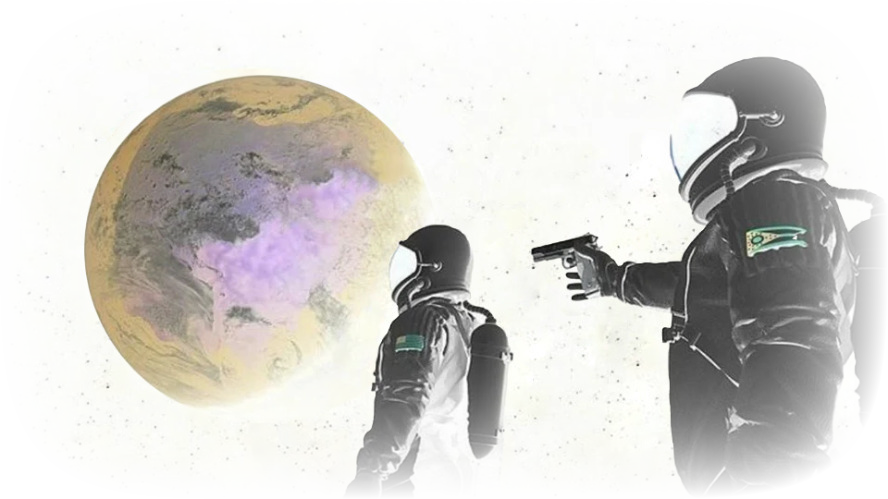
\includegraphics[width=\textwidth]{chapters/superconductivity/from bcs to conventional superconductors/pictures/always.png}
	};
	\node[anchor=center] (a) at (0,0.8) {$(\mathrm{a})$};
	\node[anchor=center] (a) at (3.8,3) {$(\mathrm{b})$};
\end{tikzpicture}
	\caption[$(\mathrm{a})$ Wait, is it a superconductor?; $(\mathrm{b})$ Always has been.]
	{\tabular[t]{@{}l@{}}$(\mathrm{a})$ Wait, is it a superconductor? \\ $(\mathrm{b})$ Always has been.\endtabular}
	\label{fig:always}
\end{figure}